\documentclass[1p]{elsarticle_modified}
%\bibliographystyle{elsarticle-num}

%\usepackage[colorlinks]{hyperref}
%\usepackage{abbrmath_seonhwa} %\Abb, \Ascr, \Acal ,\Abf, \Afrak
\usepackage{amsfonts}
\usepackage{amssymb}
\usepackage{amsmath}
\usepackage{amsthm}
\usepackage{scalefnt}
\usepackage{amsbsy}
\usepackage{kotex}
\usepackage{caption}
\usepackage{subfig}
\usepackage{color}
\usepackage{graphicx}
\usepackage{xcolor} %% white, black, red, green, blue, cyan, magenta, yellow
\usepackage{float}
\usepackage{setspace}
\usepackage{hyperref}

\usepackage{tikz}
\usetikzlibrary{arrows}

\usepackage{multirow}
\usepackage{array} % fixed length table
\usepackage{hhline}

%%%%%%%%%%%%%%%%%%%%%
\makeatletter
\renewcommand*\env@matrix[1][\arraystretch]{%
	\edef\arraystretch{#1}%
	\hskip -\arraycolsep
	\let\@ifnextchar\new@ifnextchar
	\array{*\c@MaxMatrixCols c}}
\makeatother %https://tex.stackexchange.com/questions/14071/how-can-i-increase-the-line-spacing-in-a-matrix
%%%%%%%%%%%%%%%

\usepackage[normalem]{ulem}

\newcommand{\msout}[1]{\ifmmode\text{\sout{\ensuremath{#1}}}\else\sout{#1}\fi}
%SOURCE: \msout is \stkout macro in https://tex.stackexchange.com/questions/20609/strikeout-in-math-mode

\newcommand{\cancel}[1]{
	\ifmmode
	{\color{red}\msout{#1}}
	\else
	{\color{red}\sout{#1}}
	\fi
}

\newcommand{\add}[1]{
	{\color{blue}\uwave{#1}}
}

\newcommand{\replace}[2]{
	\ifmmode
	{\color{red}\msout{#1}}{\color{blue}\uwave{#2}}
	\else
	{\color{red}\sout{#1}}{\color{blue}\uwave{#2}}
	\fi
}

\newcommand{\Sol}{\mathcal{S}} %segment
\newcommand{\D}{D} %diagram
\newcommand{\A}{\mathcal{A}} %arc


%%%%%%%%%%%%%%%%%%%%%%%%%%%%%5 test

\def\sl{\operatorname{\textup{SL}}(2,\Cbb)}
\def\psl{\operatorname{\textup{PSL}}(2,\Cbb)}
\def\quan{\mkern 1mu \triangleright \mkern 1mu}

\theoremstyle{definition}
\newtheorem{thm}{Theorem}[section]
\newtheorem{prop}[thm]{Proposition}
\newtheorem{lem}[thm]{Lemma}
\newtheorem{ques}[thm]{Question}
\newtheorem{cor}[thm]{Corollary}
\newtheorem{defn}[thm]{Definition}
\newtheorem{exam}[thm]{Example}
\newtheorem{rmk}[thm]{Remark}
\newtheorem{alg}[thm]{Algorithm}

\newcommand{\I}{\sqrt{-1}}
\begin{document}

%\begin{frontmatter}
%
%\title{Boundary parabolic representations of knots up to 8 crossings}
%
%%% Group authors per affiliation:
%\author{Yunhi Cho} 
%\address{Department of Mathematics, University of Seoul, Seoul, Korea}
%\ead{yhcho@uos.ac.kr}
%
%
%\author{Seonhwa Kim} %\fnref{s_kim}}
%\address{Center for Geometry and Physics, Institute for Basic Science, Pohang, 37673, Korea}
%\ead{ryeona17@ibs.re.kr}
%
%\author{Hyuk Kim}
%\address{Department of Mathematical Sciences, Seoul National University, Seoul 08826, Korea}
%\ead{hyukkim@snu.ac.kr}
%
%\author{Seokbeom Yoon}
%\address{Department of Mathematical Sciences, Seoul National University, Seoul, 08826,  Korea}
%\ead{sbyoon15@snu.ac.kr}
%
%\begin{abstract}
%We find all boundary parabolic representation of knots up to 8 crossings.
%
%\end{abstract}
%\begin{keyword}
%    \MSC[2010] 57M25 
%\end{keyword}
%
%\end{frontmatter}

%\linenumbers
%\tableofcontents
%
\newcommand\colored[1]{\textcolor{white}{\rule[-0.35ex]{0.8em}{1.4ex}}\kern-0.8em\color{red} #1}%
%\newcommand\colored[1]{\textcolor{white}{ #1}\kern-2.17ex	\textcolor{white}{ #1}\kern-1.81ex	\textcolor{white}{ #1}\kern-2.15ex\color{red}#1	}

{\Large $\underline{12n_{0784}~(K12n_{0784})}$}

\setlength{\tabcolsep}{10pt}
\renewcommand{\arraystretch}{1.6}
\vspace{1cm}\begin{tabular}{m{100pt}>{\centering\arraybackslash}m{274pt}}
\multirow{5}{120pt}{
	\centering
	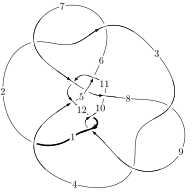
\includegraphics[width=112pt]{../../../GIT/diagram.site/Diagrams/png/2873_12n_0784.png}\\
\ \ \ A knot diagram\footnotemark}&
\allowdisplaybreaks
\textbf{Linearized knot diagam} \\
\cline{2-2}
 &
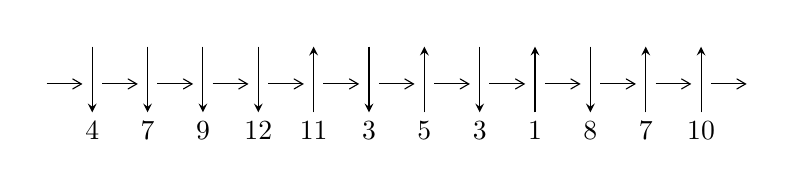
\begin{tikzpicture}[x=20pt, y=17pt]
	% nodes
	\node (C0) at (0, 0) {};
	\node (C1) at (1, 0) {};
	\node (C1U) at (1, +1) {};
	\node (C1D) at (1, -1) {4};

	\node (C2) at (2, 0) {};
	\node (C2U) at (2, +1) {};
	\node (C2D) at (2, -1) {7};

	\node (C3) at (3, 0) {};
	\node (C3U) at (3, +1) {};
	\node (C3D) at (3, -1) {9};

	\node (C4) at (4, 0) {};
	\node (C4U) at (4, +1) {};
	\node (C4D) at (4, -1) {12};

	\node (C5) at (5, 0) {};
	\node (C5U) at (5, +1) {};
	\node (C5D) at (5, -1) {11};

	\node (C6) at (6, 0) {};
	\node (C6U) at (6, +1) {};
	\node (C6D) at (6, -1) {3};

	\node (C7) at (7, 0) {};
	\node (C7U) at (7, +1) {};
	\node (C7D) at (7, -1) {5};

	\node (C8) at (8, 0) {};
	\node (C8U) at (8, +1) {};
	\node (C8D) at (8, -1) {3};

	\node (C9) at (9, 0) {};
	\node (C9U) at (9, +1) {};
	\node (C9D) at (9, -1) {1};

	\node (C10) at (10, 0) {};
	\node (C10U) at (10, +1) {};
	\node (C10D) at (10, -1) {8};

	\node (C11) at (11, 0) {};
	\node (C11U) at (11, +1) {};
	\node (C11D) at (11, -1) {7};

	\node (C12) at (12, 0) {};
	\node (C12U) at (12, +1) {};
	\node (C12D) at (12, -1) {10};
	\node (C13) at (13, 0) {};

	% arrows
	\draw[->,>={angle 60}]
	(C0) edge (C1) (C1) edge (C2) (C2) edge (C3) (C3) edge (C4) (C4) edge (C5) (C5) edge (C6) (C6) edge (C7) (C7) edge (C8) (C8) edge (C9) (C9) edge (C10) (C10) edge (C11) (C11) edge (C12) (C12) edge (C13) ;	\draw[->,>=stealth]
	(C1U) edge (C1D) (C2U) edge (C2D) (C3U) edge (C3D) (C4U) edge (C4D) (C5D) edge (C5U) (C6U) edge (C6D) (C7D) edge (C7U) (C8U) edge (C8D) (C9D) edge (C9U) (C10U) edge (C10D) (C11D) edge (C11U) (C12D) edge (C12U) ;
	\end{tikzpicture} \\
\hhline{~~} \\& 
\textbf{Solving Sequence} \\ \cline{2-2} 
 &
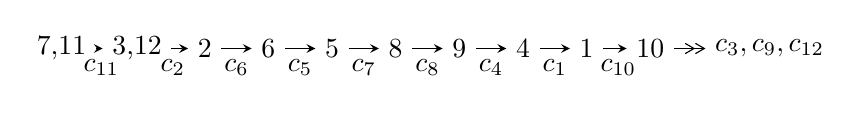
\begin{tikzpicture}[x=23pt, y=7pt]
	% node
	\node (A0) at (-1/8, 0) {7,11};
	\node (A1) at (17/16, 0) {3,12};
	\node (A2) at (17/8, 0) {2};
	\node (A3) at (25/8, 0) {6};
	\node (A4) at (33/8, 0) {5};
	\node (A5) at (41/8, 0) {8};
	\node (A6) at (49/8, 0) {9};
	\node (A7) at (57/8, 0) {4};
	\node (A8) at (65/8, 0) {1};
	\node (A9) at (73/8, 0) {10};
	\node (C1) at (1/2, -1) {$c_{11}$};
	\node (C2) at (13/8, -1) {$c_{2}$};
	\node (C3) at (21/8, -1) {$c_{6}$};
	\node (C4) at (29/8, -1) {$c_{5}$};
	\node (C5) at (37/8, -1) {$c_{7}$};
	\node (C6) at (45/8, -1) {$c_{8}$};
	\node (C7) at (53/8, -1) {$c_{4}$};
	\node (C8) at (61/8, -1) {$c_{1}$};
	\node (C9) at (69/8, -1) {$c_{10}$};
	\node (A10) at (11, 0) {$c_{3},c_{9},c_{12}$};

	% edge
	\draw[->,>=stealth]	
	(A0) edge (A1) (A1) edge (A2) (A2) edge (A3) (A3) edge (A4) (A4) edge (A5) (A5) edge (A6) (A6) edge (A7) (A7) edge (A8) (A8) edge (A9) ;
	\draw[->>,>={angle 60}]	
	(A9) edge (A10);
\end{tikzpicture} \\ 

\end{tabular} \\

\footnotetext{
The image of knot diagram is generated by the software ``\textbf{Draw programme}" developed by Andrew Bartholomew(\url{http://www.layer8.co.uk/maths/draw/index.htm\#Running-draw}), where we modified some parts for our purpose(\url{https://github.com/CATsTAILs/LinksPainter}).
}\phantom \\ \newline 
\centering \textbf{Ideals for irreducible components\footnotemark of $X_{\text{par}}$} 
 
\begin{align*}
I^u_{1}&=\langle 
-3.76991\times10^{683} u^{96}-1.11129\times10^{684} u^{95}+\cdots+2.93219\times10^{689} b-1.43801\times10^{689},\\
\phantom{I^u_{1}}&\phantom{= \langle  }-3.81255\times10^{687} u^{96}-1.08815\times10^{688} u^{95}+\cdots+3.67491\times10^{692} a-3.18684\times10^{693},\\
\phantom{I^u_{1}}&\phantom{= \langle  }u^{97}+3 u^{96}+\cdots-326815 u+423614\rangle \\
I^u_{2}&=\langle 
-2.33693\times10^{55} u^{35}-1.33989\times10^{54} u^{34}+\cdots+2.94617\times10^{55} b+8.02253\times10^{54},\\
\phantom{I^u_{2}}&\phantom{= \langle  }-7.16188\times10^{55} u^{35}-1.46151\times10^{55} u^{34}+\cdots+2.94617\times10^{55} a+9.34411\times10^{55},\;u^{36}-7 u^{34}+\cdots-2 u-1\rangle \\
\\
\end{align*}
\raggedright * 2 irreducible components of $\dim_{\mathbb{C}}=0$, with total 133 representations.\\
\footnotetext{All coefficients of polynomials are rational numbers. But the coefficients are sometimes approximated in decimal forms when there is not enough margin.}
\newpage
\renewcommand{\arraystretch}{1}
\centering \section*{I. $I^u_{1}= \langle -3.77\times10^{683} u^{96}-1.11\times10^{684} u^{95}+\cdots+2.93\times10^{689} b-1.44\times10^{689},\;-3.81\times10^{687} u^{96}-1.09\times10^{688} u^{95}+\cdots+3.67\times10^{692} a-3.19\times10^{693},\;u^{97}+3 u^{96}+\cdots-326815 u+423614 \rangle$}
\flushleft \textbf{(i) Arc colorings}\\
\begin{tabular}{m{7pt} m{180pt} m{7pt} m{180pt} }
\flushright $a_{7}=$&$\begin{pmatrix}0\\u\end{pmatrix}$ \\
\flushright $a_{11}=$&$\begin{pmatrix}1\\0\end{pmatrix}$ \\
\flushright $a_{3}=$&$\begin{pmatrix}0.0000103746 u^{96}+0.0000296103 u^{95}+\cdots-5.13025 u+8.67190\\1.28570\times10^{-6} u^{96}+3.78995\times10^{-6} u^{95}+\cdots+1.97339 u+0.490420\end{pmatrix}$ \\
\flushright $a_{12}=$&$\begin{pmatrix}1\\- u^2\end{pmatrix}$ \\
\flushright $a_{2}=$&$\begin{pmatrix}0.0000103746 u^{96}+0.0000296103 u^{95}+\cdots-5.13025 u+8.67190\\3.02293\times10^{-6} u^{96}+7.99155\times10^{-6} u^{95}+\cdots+6.86279 u-0.150671\end{pmatrix}$ \\
\flushright $a_{6}=$&$\begin{pmatrix}7.84420\times10^{-6} u^{96}+0.0000208910 u^{95}+\cdots+12.2774 u+1.57910\\4.97744\times10^{-8} u^{96}+8.34988\times10^{-8} u^{95}+\cdots+0.288331 u+0.473383\end{pmatrix}$ \\
\flushright $a_{5}=$&$\begin{pmatrix}7.79443\times10^{-6} u^{96}+0.0000208075 u^{95}+\cdots+11.9891 u+1.10572\\4.97744\times10^{-8} u^{96}+8.34988\times10^{-8} u^{95}+\cdots+0.288331 u+0.473383\end{pmatrix}$ \\
\flushright $a_{8}=$&$\begin{pmatrix}-0.0000204260 u^{96}-0.0000572511 u^{95}+\cdots-27.5893 u-6.39711\\1.61577\times10^{-6} u^{96}+4.87046\times10^{-6} u^{95}+\cdots+2.05769 u+1.46957\end{pmatrix}$ \\
\flushright $a_{9}=$&$\begin{pmatrix}-9.88886\times10^{-6} u^{96}-0.0000265271 u^{95}+\cdots-21.3728 u+0.115127\\-9.04866\times10^{-7} u^{96}-2.45873\times10^{-6} u^{95}+\cdots-0.780709 u+0.557878\end{pmatrix}$ \\
\flushright $a_{4}=$&$\begin{pmatrix}6.73434\times10^{-6} u^{96}+0.0000187268 u^{95}+\cdots+8.13376 u+2.67026\\7.03433\times10^{-8} u^{96}+2.51508\times10^{-7} u^{95}+\cdots-0.520092 u+0.939174\end{pmatrix}$ \\
\flushright $a_{1}=$&$\begin{pmatrix}3.07647\times10^{-6} u^{96}+7.59451\times10^{-6} u^{95}+\cdots+12.1478 u-2.13295\\-2.32077\times10^{-6} u^{96}-6.97629\times10^{-6} u^{95}+\cdots-2.64506 u-0.636660\end{pmatrix}$ \\
\flushright $a_{10}=$&$\begin{pmatrix}4.36241\times10^{-6} u^{96}+0.0000116402 u^{95}+\cdots+12.3313 u+0.259494\\3.20577\times10^{-8} u^{96}+2.63754\times10^{-7} u^{95}+\cdots+0.735310 u+0.204890\end{pmatrix}$\\&\end{tabular}
\flushleft \textbf{(ii) Obstruction class $= -1$}\\~\\
\flushleft \textbf{(iii) Cusp Shapes $= 0.0000318183 u^{96}+0.0000744702 u^{95}+\cdots+139.903 u-26.7053$}\\~\\
\newpage\renewcommand{\arraystretch}{1}
\flushleft \textbf{(iv) u-Polynomials at the component}\newline \\
\begin{tabular}{m{50pt}|m{274pt}}
Crossings & \hspace{64pt}u-Polynomials at each crossing \\
\hline $$\begin{aligned}c_{1}\end{aligned}$$&$\begin{aligned}
&u^{97}-6 u^{96}+\cdots+11484641 u+1234962
\end{aligned}$\\
\hline $$\begin{aligned}c_{2},c_{6}\end{aligned}$$&$\begin{aligned}
&u^{97}+3 u^{96}+\cdots+38 u-1
\end{aligned}$\\
\hline $$\begin{aligned}c_{3},c_{8}\end{aligned}$$&$\begin{aligned}
&u^{97}- u^{96}+\cdots-45431 u+10369
\end{aligned}$\\
\hline $$\begin{aligned}c_{4}\end{aligned}$$&$\begin{aligned}
&u^{97}+3 u^{96}+\cdots-524325 u+114823
\end{aligned}$\\
\hline $$\begin{aligned}c_{5}\end{aligned}$$&$\begin{aligned}
&u^{97}+u^{96}+\cdots+4369766 u-1681359
\end{aligned}$\\
\hline $$\begin{aligned}c_{7}\end{aligned}$$&$\begin{aligned}
&u^{97}+9 u^{96}+\cdots+6 u+1
\end{aligned}$\\
\hline $$\begin{aligned}c_{9},c_{12}\end{aligned}$$&$\begin{aligned}
&u^{97}-4 u^{96}+\cdots+858 u+53
\end{aligned}$\\
\hline $$\begin{aligned}c_{10}\end{aligned}$$&$\begin{aligned}
&u^{97}-9 u^{96}+\cdots-766766 u+291457
\end{aligned}$\\
\hline $$\begin{aligned}c_{11}\end{aligned}$$&$\begin{aligned}
&u^{97}-3 u^{96}+\cdots-326815 u-423614
\end{aligned}$\\
\hline
\end{tabular}\\~\\
\newpage\renewcommand{\arraystretch}{1}
\flushleft \textbf{(v) Riley Polynomials at the component}\newline \\
\begin{tabular}{m{50pt}|m{274pt}}
Crossings & \hspace{64pt}Riley Polynomials at each crossing \\
\hline $$\begin{aligned}c_{1}\end{aligned}$$&$\begin{aligned}
&y^{97}-56 y^{96}+\cdots+104656278490069 y-1525131141444
\end{aligned}$\\
\hline $$\begin{aligned}c_{2},c_{6}\end{aligned}$$&$\begin{aligned}
&y^{97}-87 y^{96}+\cdots+162 y-1
\end{aligned}$\\
\hline $$\begin{aligned}c_{3},c_{8}\end{aligned}$$&$\begin{aligned}
&y^{97}-99 y^{96}+\cdots+13533582897 y-107516161
\end{aligned}$\\
\hline $$\begin{aligned}c_{4}\end{aligned}$$&$\begin{aligned}
&y^{97}-7 y^{96}+\cdots-204662681307 y-13184321329
\end{aligned}$\\
\hline $$\begin{aligned}c_{5}\end{aligned}$$&$\begin{aligned}
&y^{97}+33 y^{96}+\cdots-52295137112108 y-2826968086881
\end{aligned}$\\
\hline $$\begin{aligned}c_{7}\end{aligned}$$&$\begin{aligned}
&y^{97}-23 y^{96}+\cdots+72 y-1
\end{aligned}$\\
\hline $$\begin{aligned}c_{9},c_{12}\end{aligned}$$&$\begin{aligned}
&y^{97}+64 y^{96}+\cdots+894104 y-2809
\end{aligned}$\\
\hline $$\begin{aligned}c_{10}\end{aligned}$$&$\begin{aligned}
&y^{97}-45 y^{96}+\cdots+2453858214746 y-84947182849
\end{aligned}$\\
\hline $$\begin{aligned}c_{11}\end{aligned}$$&$\begin{aligned}
&y^{97}+25 y^{96}+\cdots-3682305657223 y-179448820996
\end{aligned}$\\
\hline
\end{tabular}\\~\\
\newpage\flushleft \textbf{(vi) Complex Volumes and Cusp Shapes}
$$\begin{array}{c|c|c}  
\text{Solutions to }I^u_{1}& \I (\text{vol} + \sqrt{-1}CS) & \text{Cusp shape}\\
 \hline 
\begin{aligned}
u &= \phantom{-}0.923522 + 0.419939 I \\
a &= -0.141190 - 0.711239 I \\
b &= -0.213610 + 0.164942 I\end{aligned}
 & \phantom{-}1.63907 + 6.49597 I & \phantom{-0.000000 } 0 \\ \hline\begin{aligned}
u &= \phantom{-}0.923522 - 0.419939 I \\
a &= -0.141190 + 0.711239 I \\
b &= -0.213610 - 0.164942 I\end{aligned}
 & \phantom{-}1.63907 - 6.49597 I & \phantom{-0.000000 } 0 \\ \hline\begin{aligned}
u &= -0.862563 + 0.538663 I \\
a &= \phantom{-}0.487071 - 0.589429 I \\
b &= -0.034290 + 0.213039 I\end{aligned}
 & \phantom{-}2.83107 - 2.04200 I & \phantom{-0.000000 } 0 \\ \hline\begin{aligned}
u &= -0.862563 - 0.538663 I \\
a &= \phantom{-}0.487071 + 0.589429 I \\
b &= -0.034290 - 0.213039 I\end{aligned}
 & \phantom{-}2.83107 + 2.04200 I & \phantom{-0.000000 } 0 \\ \hline\begin{aligned}
u &= -0.940702 + 0.267807 I \\
a &= \phantom{-}0.358836 - 0.095616 I \\
b &= -0.489850 + 0.448270 I\end{aligned}
 & \phantom{-}1.59879 - 0.37419 I & \phantom{-0.000000 } 0 \\ \hline\begin{aligned}
u &= -0.940702 - 0.267807 I \\
a &= \phantom{-}0.358836 + 0.095616 I \\
b &= -0.489850 - 0.448270 I\end{aligned}
 & \phantom{-}1.59879 + 0.37419 I & \phantom{-0.000000 } 0 \\ \hline\begin{aligned}
u &= \phantom{-}0.647383 + 0.723678 I \\
a &= -0.307654 - 0.408777 I \\
b &= \phantom{-}0.488257 + 0.100321 I\end{aligned}
 & -2.76377 + 2.06605 I & \phantom{-0.000000 } 0 \\ \hline\begin{aligned}
u &= \phantom{-}0.647383 - 0.723678 I \\
a &= -0.307654 + 0.408777 I \\
b &= \phantom{-}0.488257 - 0.100321 I\end{aligned}
 & -2.76377 - 2.06605 I & \phantom{-0.000000 } 0 \\ \hline\begin{aligned}
u &= -0.640499 + 0.727294 I \\
a &= -0.810670 - 0.913479 I \\
b &= -0.65070 - 1.54938 I\end{aligned}
 & -3.99650 - 2.93403 I & \phantom{-0.000000 } 0 \\ \hline\begin{aligned}
u &= -0.640499 - 0.727294 I \\
a &= -0.810670 + 0.913479 I \\
b &= -0.65070 + 1.54938 I\end{aligned}
 & -3.99650 + 2.93403 I & \phantom{-0.000000 } 0\\
 \hline 
 \end{array}$$\newpage$$\begin{array}{c|c|c}  
\text{Solutions to }I^u_{1}& \I (\text{vol} + \sqrt{-1}CS) & \text{Cusp shape}\\
 \hline 
\begin{aligned}
u &= \phantom{-}0.574971 + 0.879011 I \\
a &= -0.706880 + 1.199510 I \\
b &= \phantom{-}0.59602 + 1.67422 I\end{aligned}
 & -4.82694 + 4.90372 I & \phantom{-0.000000 } 0 \\ \hline\begin{aligned}
u &= \phantom{-}0.574971 - 0.879011 I \\
a &= -0.706880 - 1.199510 I \\
b &= \phantom{-}0.59602 - 1.67422 I\end{aligned}
 & -4.82694 - 4.90372 I & \phantom{-0.000000 } 0 \\ \hline\begin{aligned}
u &= -0.923843 + 0.563679 I \\
a &= -0.042756 - 0.154213 I \\
b &= \phantom{-}1.18616 - 0.87947 I\end{aligned}
 & -5.75571 - 6.53782 I & \phantom{-0.000000 } 0 \\ \hline\begin{aligned}
u &= -0.923843 - 0.563679 I \\
a &= -0.042756 + 0.154213 I \\
b &= \phantom{-}1.18616 + 0.87947 I\end{aligned}
 & -5.75571 + 6.53782 I & \phantom{-0.000000 } 0 \\ \hline\begin{aligned}
u &= \phantom{-}0.116869 + 1.092610 I \\
a &= -0.17809 + 1.48324 I \\
b &= -0.57730 + 1.81085 I\end{aligned}
 & -12.5963 - 6.5769 I & \phantom{-0.000000 } 0 \\ \hline\begin{aligned}
u &= \phantom{-}0.116869 - 1.092610 I \\
a &= -0.17809 - 1.48324 I \\
b &= -0.57730 - 1.81085 I\end{aligned}
 & -12.5963 + 6.5769 I & \phantom{-0.000000 } 0 \\ \hline\begin{aligned}
u &= -0.125613 + 0.891330 I \\
a &= -0.0640181 + 0.0757123 I \\
b &= \phantom{-}2.59653 + 0.53168 I\end{aligned}
 & -2.89330 + 7.74015 I & -15.9250 - 4.6761 I \\ \hline\begin{aligned}
u &= -0.125613 - 0.891330 I \\
a &= -0.0640181 - 0.0757123 I \\
b &= \phantom{-}2.59653 - 0.53168 I\end{aligned}
 & -2.89330 - 7.74015 I & -15.9250 + 4.6761 I \\ \hline\begin{aligned}
u &= \phantom{-}0.415341 + 1.062690 I \\
a &= \phantom{-}0.609307 - 1.263920 I \\
b &= -0.39602 - 1.44832 I\end{aligned}
 & -4.29659 + 2.89746 I & \phantom{-0.000000 } 0 \\ \hline\begin{aligned}
u &= \phantom{-}0.415341 - 1.062690 I \\
a &= \phantom{-}0.609307 + 1.263920 I \\
b &= -0.39602 + 1.44832 I\end{aligned}
 & -4.29659 - 2.89746 I & \phantom{-0.000000 } 0\\
 \hline 
 \end{array}$$\newpage$$\begin{array}{c|c|c}  
\text{Solutions to }I^u_{1}& \I (\text{vol} + \sqrt{-1}CS) & \text{Cusp shape}\\
 \hline 
\begin{aligned}
u &= -0.006624 + 0.851226 I \\
a &= -0.28218 - 1.60423 I \\
b &= \phantom{-}0.41444 - 1.42814 I\end{aligned}
 & -2.89748 + 0.28298 I & -2.00000 - 1.27836 I \\ \hline\begin{aligned}
u &= -0.006624 - 0.851226 I \\
a &= -0.28218 + 1.60423 I \\
b &= \phantom{-}0.41444 + 1.42814 I\end{aligned}
 & -2.89748 - 0.28298 I & -2.00000 + 1.27836 I \\ \hline\begin{aligned}
u &= \phantom{-}0.602528 + 0.597332 I \\
a &= -1.017100 + 0.021901 I \\
b &= \phantom{-}0.844467 + 0.976107 I\end{aligned}
 & -0.58135 - 4.78436 I & -7.16761 + 8.69455 I \\ \hline\begin{aligned}
u &= \phantom{-}0.602528 - 0.597332 I \\
a &= -1.017100 - 0.021901 I \\
b &= \phantom{-}0.844467 - 0.976107 I\end{aligned}
 & -0.58135 + 4.78436 I & -7.16761 - 8.69455 I \\ \hline\begin{aligned}
u &= -0.398228 + 1.092810 I \\
a &= -1.077510 + 0.417394 I \\
b &= -0.0958419 - 0.0506402 I\end{aligned}
 & -8.13927 + 2.05497 I & \phantom{-0.000000 } 0 \\ \hline\begin{aligned}
u &= -0.398228 - 1.092810 I \\
a &= -1.077510 - 0.417394 I \\
b &= -0.0958419 + 0.0506402 I\end{aligned}
 & -8.13927 - 2.05497 I & \phantom{-0.000000 } 0 \\ \hline\begin{aligned}
u &= \phantom{-}1.156450 + 0.156568 I \\
a &= \phantom{-}0.278185 - 0.941968 I \\
b &= -0.09792 - 2.37813 I\end{aligned}
 & \phantom{-}1.77212 + 4.10712 I & \phantom{-0.000000 } 0 \\ \hline\begin{aligned}
u &= \phantom{-}1.156450 - 0.156568 I \\
a &= \phantom{-}0.278185 + 0.941968 I \\
b &= -0.09792 + 2.37813 I\end{aligned}
 & \phantom{-}1.77212 - 4.10712 I & \phantom{-0.000000 } 0 \\ \hline\begin{aligned}
u &= \phantom{-}1.105100 + 0.379840 I \\
a &= -0.182877 - 0.225699 I \\
b &= -0.022022 - 0.775036 I\end{aligned}
 & -0.18199 + 3.83962 I & \phantom{-0.000000 } 0 \\ \hline\begin{aligned}
u &= \phantom{-}1.105100 - 0.379840 I \\
a &= -0.182877 + 0.225699 I \\
b &= -0.022022 + 0.775036 I\end{aligned}
 & -0.18199 - 3.83962 I & \phantom{-0.000000 } 0\\
 \hline 
 \end{array}$$\newpage$$\begin{array}{c|c|c}  
\text{Solutions to }I^u_{1}& \I (\text{vol} + \sqrt{-1}CS) & \text{Cusp shape}\\
 \hline 
\begin{aligned}
u &= -0.066796 + 0.797343 I \\
a &= \phantom{-}0.0190218 + 0.1360920 I \\
b &= -1.86362 + 1.01515 I\end{aligned}
 & \phantom{-}2.50193 - 2.22011 I & -4.88704 + 9.89983 I \\ \hline\begin{aligned}
u &= -0.066796 - 0.797343 I \\
a &= \phantom{-}0.0190218 - 0.1360920 I \\
b &= -1.86362 - 1.01515 I\end{aligned}
 & \phantom{-}2.50193 + 2.22011 I & -4.88704 - 9.89983 I \\ \hline\begin{aligned}
u &= \phantom{-}1.182660 + 0.204302 I \\
a &= -0.257969 - 0.155904 I \\
b &= \phantom{-}0.230698 - 0.885742 I\end{aligned}
 & -0.14085 + 3.92471 I & \phantom{-0.000000 } 0 \\ \hline\begin{aligned}
u &= \phantom{-}1.182660 - 0.204302 I \\
a &= -0.257969 + 0.155904 I \\
b &= \phantom{-}0.230698 + 0.885742 I\end{aligned}
 & -0.14085 - 3.92471 I & \phantom{-0.000000 } 0 \\ \hline\begin{aligned}
u &= \phantom{-}0.579912 + 1.053320 I \\
a &= -0.05703 + 1.48597 I \\
b &= \phantom{-}0.02168 + 1.42488 I\end{aligned}
 & -12.5183 + 9.8935 I & \phantom{-0.000000 } 0 \\ \hline\begin{aligned}
u &= \phantom{-}0.579912 - 1.053320 I \\
a &= -0.05703 - 1.48597 I \\
b &= \phantom{-}0.02168 - 1.42488 I\end{aligned}
 & -12.5183 - 9.8935 I & \phantom{-0.000000 } 0 \\ \hline\begin{aligned}
u &= \phantom{-}0.795290 + 0.028539 I \\
a &= \phantom{-}1.122040 + 0.246087 I \\
b &= \phantom{-}0.633574 + 0.435374 I\end{aligned}
 & -0.836585 + 0.106654 I & -8.30547 - 5.66017 I \\ \hline\begin{aligned}
u &= \phantom{-}0.795290 - 0.028539 I \\
a &= \phantom{-}1.122040 - 0.246087 I \\
b &= \phantom{-}0.633574 - 0.435374 I\end{aligned}
 & -0.836585 - 0.106654 I & -8.30547 + 5.66017 I \\ \hline\begin{aligned}
u &= -1.21270\phantom{ +0.000000I} \\
a &= \phantom{-}1.38716\phantom{ +0.000000I} \\
b &= \phantom{-}0.991209\phantom{ +0.000000I}\end{aligned}
 & -3.84308\phantom{ +0.000000I} & \phantom{-0.000000 } 0 \\ \hline\begin{aligned}
u &= \phantom{-}0.281235 + 0.719483 I \\
a &= \phantom{-}0.028419 + 0.260896 I \\
b &= \phantom{-}1.091930 + 0.404289 I\end{aligned}
 & \phantom{-}0.03454 - 3.03484 I & -2.77691 + 0.64392 I\\
 \hline 
 \end{array}$$\newpage$$\begin{array}{c|c|c}  
\text{Solutions to }I^u_{1}& \I (\text{vol} + \sqrt{-1}CS) & \text{Cusp shape}\\
 \hline 
\begin{aligned}
u &= \phantom{-}0.281235 - 0.719483 I \\
a &= \phantom{-}0.028419 - 0.260896 I \\
b &= \phantom{-}1.091930 - 0.404289 I\end{aligned}
 & \phantom{-}0.03454 + 3.03484 I & -2.77691 - 0.64392 I \\ \hline\begin{aligned}
u &= \phantom{-}1.141950 + 0.454769 I \\
a &= -1.221940 + 0.431608 I \\
b &= -0.873299 + 0.669264 I\end{aligned}
 & -8.50791 + 7.03123 I & \phantom{-0.000000 } 0 \\ \hline\begin{aligned}
u &= \phantom{-}1.141950 - 0.454769 I \\
a &= -1.221940 - 0.431608 I \\
b &= -0.873299 - 0.669264 I\end{aligned}
 & -8.50791 - 7.03123 I & \phantom{-0.000000 } 0 \\ \hline\begin{aligned}
u &= -0.378164 + 1.200280 I \\
a &= \phantom{-}0.011811 - 1.286790 I \\
b &= -0.310358 - 1.324910 I\end{aligned}
 & -6.56438 - 2.28949 I & \phantom{-0.000000 } 0 \\ \hline\begin{aligned}
u &= -0.378164 - 1.200280 I \\
a &= \phantom{-}0.011811 + 1.286790 I \\
b &= -0.310358 + 1.324910 I\end{aligned}
 & -6.56438 + 2.28949 I & \phantom{-0.000000 } 0 \\ \hline\begin{aligned}
u &= \phantom{-}0.028117 + 0.736591 I \\
a &= -0.08855 + 2.18812 I \\
b &= \phantom{-}0.25582 + 1.90745 I\end{aligned}
 & -5.81101 + 3.05040 I & -1.70242 - 4.94793 I \\ \hline\begin{aligned}
u &= \phantom{-}0.028117 - 0.736591 I \\
a &= -0.08855 - 2.18812 I \\
b &= \phantom{-}0.25582 - 1.90745 I\end{aligned}
 & -5.81101 - 3.05040 I & -1.70242 + 4.94793 I \\ \hline\begin{aligned}
u &= -0.425850 + 1.198780 I \\
a &= -0.104106 + 1.361580 I \\
b &= \phantom{-}0.04697 + 1.50054 I\end{aligned}
 & -8.43987 - 4.77545 I & \phantom{-0.000000 } 0 \\ \hline\begin{aligned}
u &= -0.425850 - 1.198780 I \\
a &= -0.104106 - 1.361580 I \\
b &= \phantom{-}0.04697 - 1.50054 I\end{aligned}
 & -8.43987 + 4.77545 I & \phantom{-0.000000 } 0 \\ \hline\begin{aligned}
u &= -1.033450 + 0.798470 I \\
a &= \phantom{-}0.730998 + 0.691800 I \\
b &= -0.83004 + 1.69639 I\end{aligned}
 & -5.67762 - 6.64568 I & \phantom{-0.000000 } 0\\
 \hline 
 \end{array}$$\newpage$$\begin{array}{c|c|c}  
\text{Solutions to }I^u_{1}& \I (\text{vol} + \sqrt{-1}CS) & \text{Cusp shape}\\
 \hline 
\begin{aligned}
u &= -1.033450 - 0.798470 I \\
a &= \phantom{-}0.730998 - 0.691800 I \\
b &= -0.83004 - 1.69639 I\end{aligned}
 & -5.67762 + 6.64568 I & \phantom{-0.000000 } 0 \\ \hline\begin{aligned}
u &= \phantom{-}0.617943 + 0.301216 I \\
a &= \phantom{-}0.34881 - 1.60123 I \\
b &= \phantom{-}0.582353 - 0.610573 I\end{aligned}
 & -2.48190 + 3.88876 I & -6.60825 - 4.23609 I \\ \hline\begin{aligned}
u &= \phantom{-}0.617943 - 0.301216 I \\
a &= \phantom{-}0.34881 + 1.60123 I \\
b &= \phantom{-}0.582353 + 0.610573 I\end{aligned}
 & -2.48190 - 3.88876 I & -6.60825 + 4.23609 I \\ \hline\begin{aligned}
u &= -0.541139 + 0.299003 I \\
a &= \phantom{-}0.566676 - 0.958665 I \\
b &= -0.903463 + 0.302588 I\end{aligned}
 & \phantom{-}1.87171 - 0.57875 I & \phantom{-}2.53846 + 0.89508 I \\ \hline\begin{aligned}
u &= -0.541139 - 0.299003 I \\
a &= \phantom{-}0.566676 + 0.958665 I \\
b &= -0.903463 - 0.302588 I\end{aligned}
 & \phantom{-}1.87171 + 0.57875 I & \phantom{-}2.53846 - 0.89508 I \\ \hline\begin{aligned}
u &= -1.25310 + 0.70769 I \\
a &= \phantom{-}0.303565 - 0.312300 I \\
b &= -0.378188 - 0.451986 I\end{aligned}
 & -1.93093 - 4.24065 I & \phantom{-0.000000 } 0 \\ \hline\begin{aligned}
u &= -1.25310 - 0.70769 I \\
a &= \phantom{-}0.303565 + 0.312300 I \\
b &= -0.378188 + 0.451986 I\end{aligned}
 & -1.93093 + 4.24065 I & \phantom{-0.000000 } 0 \\ \hline\begin{aligned}
u &= -0.298035 + 0.440845 I \\
a &= -1.21985 - 2.03266 I \\
b &= \phantom{-}0.327599 - 1.361730 I\end{aligned}
 & -3.15077 - 0.32600 I & -3.31381 - 0.20621 I \\ \hline\begin{aligned}
u &= -0.298035 - 0.440845 I \\
a &= -1.21985 + 2.03266 I \\
b &= \phantom{-}0.327599 + 1.361730 I\end{aligned}
 & -3.15077 + 0.32600 I & -3.31381 + 0.20621 I \\ \hline\begin{aligned}
u &= \phantom{-}0.54081 + 1.38757 I \\
a &= \phantom{-}1.080280 + 0.283935 I \\
b &= \phantom{-}0.0232825 + 0.0547609 I\end{aligned}
 & -2.84867 + 2.95855 I & \phantom{-0.000000 } 0\\
 \hline 
 \end{array}$$\newpage$$\begin{array}{c|c|c}  
\text{Solutions to }I^u_{1}& \I (\text{vol} + \sqrt{-1}CS) & \text{Cusp shape}\\
 \hline 
\begin{aligned}
u &= \phantom{-}0.54081 - 1.38757 I \\
a &= \phantom{-}1.080280 - 0.283935 I \\
b &= \phantom{-}0.0232825 - 0.0547609 I\end{aligned}
 & -2.84867 - 2.95855 I & \phantom{-0.000000 } 0 \\ \hline\begin{aligned}
u &= -0.34649 + 1.46686 I \\
a &= -1.148290 + 0.269888 I \\
b &= \phantom{-}0.0407835 + 0.0416639 I\end{aligned}
 & -6.42429 - 9.16240 I & \phantom{-0.000000 } 0 \\ \hline\begin{aligned}
u &= -0.34649 - 1.46686 I \\
a &= -1.148290 - 0.269888 I \\
b &= \phantom{-}0.0407835 - 0.0416639 I\end{aligned}
 & -6.42429 + 9.16240 I & \phantom{-0.000000 } 0 \\ \hline\begin{aligned}
u &= -0.295001 + 0.378523 I \\
a &= -2.69695 + 1.42851 I \\
b &= \phantom{-}0.011606 + 0.236913 I\end{aligned}
 & \phantom{-}1.90922 + 4.76277 I & -16.1493 - 2.7551 I \\ \hline\begin{aligned}
u &= -0.295001 - 0.378523 I \\
a &= -2.69695 - 1.42851 I \\
b &= \phantom{-}0.011606 - 0.236913 I\end{aligned}
 & \phantom{-}1.90922 - 4.76277 I & -16.1493 + 2.7551 I \\ \hline\begin{aligned}
u &= -1.22798 + 0.89809 I \\
a &= -0.064238 + 0.727432 I \\
b &= -0.27578 + 2.29022 I\end{aligned}
 & \phantom{-}2.13652 - 3.54958 I & \phantom{-0.000000 } 0 \\ \hline\begin{aligned}
u &= -1.22798 - 0.89809 I \\
a &= -0.064238 - 0.727432 I \\
b &= -0.27578 - 2.29022 I\end{aligned}
 & \phantom{-}2.13652 + 3.54958 I & \phantom{-0.000000 } 0 \\ \hline\begin{aligned}
u &= \phantom{-}0.041949 + 0.445086 I \\
a &= \phantom{-}0.72714 - 1.40677 I \\
b &= -0.406883 + 0.513409 I\end{aligned}
 & -3.38531 - 0.33616 I & -6.88546 + 1.61686 I \\ \hline\begin{aligned}
u &= \phantom{-}0.041949 - 0.445086 I \\
a &= \phantom{-}0.72714 + 1.40677 I \\
b &= -0.406883 - 0.513409 I\end{aligned}
 & -3.38531 + 0.33616 I & -6.88546 - 1.61686 I \\ \hline\begin{aligned}
u &= \phantom{-}0.53757 + 1.50355 I \\
a &= \phantom{-}0.015470 + 1.161620 I \\
b &= \phantom{-}0.02277 + 1.63386 I\end{aligned}
 & -12.20690 - 0.32933 I & \phantom{-0.000000 } 0\\
 \hline 
 \end{array}$$\newpage$$\begin{array}{c|c|c}  
\text{Solutions to }I^u_{1}& \I (\text{vol} + \sqrt{-1}CS) & \text{Cusp shape}\\
 \hline 
\begin{aligned}
u &= \phantom{-}0.53757 - 1.50355 I \\
a &= \phantom{-}0.015470 - 1.161620 I \\
b &= \phantom{-}0.02277 - 1.63386 I\end{aligned}
 & -12.20690 + 0.32933 I & \phantom{-0.000000 } 0 \\ \hline\begin{aligned}
u &= -0.173989 + 0.362246 I \\
a &= \phantom{-}2.79961 - 1.61528 I \\
b &= -0.164585 + 0.163489 I\end{aligned}
 & \phantom{-}3.33787 - 1.72551 I & \phantom{-}2.6497 + 15.0642 I \\ \hline\begin{aligned}
u &= -0.173989 - 0.362246 I \\
a &= \phantom{-}2.79961 + 1.61528 I \\
b &= -0.164585 - 0.163489 I\end{aligned}
 & \phantom{-}3.33787 + 1.72551 I & \phantom{-}2.6497 - 15.0642 I \\ \hline\begin{aligned}
u &= -0.82248 + 1.42357 I \\
a &= \phantom{-}0.269489 + 0.908330 I \\
b &= -0.55475 + 1.85962 I\end{aligned}
 & -2.22870 - 6.72906 I & \phantom{-0.000000 } 0 \\ \hline\begin{aligned}
u &= -0.82248 - 1.42357 I \\
a &= \phantom{-}0.269489 - 0.908330 I \\
b &= -0.55475 - 1.85962 I\end{aligned}
 & -2.22870 + 6.72906 I & \phantom{-0.000000 } 0 \\ \hline\begin{aligned}
u &= \phantom{-}0.338771\phantom{ +0.000000I} \\
a &= \phantom{-}1.65263\phantom{ +0.000000I} \\
b &= \phantom{-}0.356841\phantom{ +0.000000I}\end{aligned}
 & -1.00609\phantom{ +0.000000I} & -10.0620\phantom{ +0.000000I} \\ \hline\begin{aligned}
u &= \phantom{-}1.04636 + 1.30233 I \\
a &= -0.359124 + 0.690834 I \\
b &= \phantom{-}0.71719 + 1.97869 I\end{aligned}
 & -6.70359 + 4.67707 I & \phantom{-0.000000 } 0 \\ \hline\begin{aligned}
u &= \phantom{-}1.04636 - 1.30233 I \\
a &= -0.359124 - 0.690834 I \\
b &= \phantom{-}0.71719 - 1.97869 I\end{aligned}
 & -6.70359 - 4.67707 I & \phantom{-0.000000 } 0 \\ \hline\begin{aligned}
u &= \phantom{-}0.65644 + 1.56802 I \\
a &= -0.204936 + 0.969419 I \\
b &= \phantom{-}0.53008 + 1.81422 I\end{aligned}
 & -5.48142 + 10.64750 I & \phantom{-0.000000 } 0 \\ \hline\begin{aligned}
u &= \phantom{-}0.65644 - 1.56802 I \\
a &= -0.204936 - 0.969419 I \\
b &= \phantom{-}0.53008 - 1.81422 I\end{aligned}
 & -5.48142 - 10.64750 I & \phantom{-0.000000 } 0\\
 \hline 
 \end{array}$$\newpage$$\begin{array}{c|c|c}  
\text{Solutions to }I^u_{1}& \I (\text{vol} + \sqrt{-1}CS) & \text{Cusp shape}\\
 \hline 
\begin{aligned}
u &= -1.07428 + 1.44140 I \\
a &= -0.153756 - 0.968831 I \\
b &= \phantom{-}0.36684 - 2.10145 I\end{aligned}
 & -12.52170 - 5.60621 I & \phantom{-0.000000 } 0 \\ \hline\begin{aligned}
u &= -1.07428 - 1.44140 I \\
a &= -0.153756 + 0.968831 I \\
b &= \phantom{-}0.36684 + 2.10145 I\end{aligned}
 & -12.52170 + 5.60621 I & \phantom{-0.000000 } 0 \\ \hline\begin{aligned}
u &= \phantom{-}1.15083 + 1.53012 I \\
a &= \phantom{-}0.203060 - 0.956730 I \\
b &= -0.38905 - 2.03922 I\end{aligned}
 & -7.62856 + 11.80710 I & \phantom{-0.000000 } 0 \\ \hline\begin{aligned}
u &= \phantom{-}1.15083 - 1.53012 I \\
a &= \phantom{-}0.203060 + 0.956730 I \\
b &= -0.38905 + 2.03922 I\end{aligned}
 & -7.62856 - 11.80710 I & \phantom{-0.000000 } 0 \\ \hline\begin{aligned}
u &= -1.16207 + 1.57256 I \\
a &= -0.221595 - 0.923585 I \\
b &= \phantom{-}0.43403 - 2.03151 I\end{aligned}
 & -11.8925 - 17.9478 I & \phantom{-0.000000 } 0 \\ \hline\begin{aligned}
u &= -1.16207 - 1.57256 I \\
a &= -0.221595 + 0.923585 I \\
b &= \phantom{-}0.43403 + 2.03151 I\end{aligned}
 & -11.8925 + 17.9478 I & \phantom{-0.000000 } 0 \\ \hline\begin{aligned}
u &= -0.10937 + 2.04865 I \\
a &= \phantom{-}0.064869 + 0.774836 I \\
b &= -0.10253 + 2.06653 I\end{aligned}
 & -10.59440 - 0.47965 I & \phantom{-0.000000 } 0 \\ \hline\begin{aligned}
u &= -0.10937 - 2.04865 I \\
a &= \phantom{-}0.064869 - 0.774836 I \\
b &= -0.10253 - 2.06653 I\end{aligned}
 & -10.59440 + 0.47965 I & \phantom{-0.000000 } 0 \\ \hline\begin{aligned}
u &= \phantom{-}0.07153 + 2.08843 I \\
a &= -0.039114 - 0.924282 I \\
b &= \phantom{-}0.08777 - 1.54467 I\end{aligned}
 & -9.10546 + 0.65646 I & \phantom{-0.000000 } 0 \\ \hline\begin{aligned}
u &= \phantom{-}0.07153 - 2.08843 I \\
a &= -0.039114 + 0.924282 I \\
b &= \phantom{-}0.08777 + 1.54467 I\end{aligned}
 & -9.10546 - 0.65646 I & \phantom{-0.000000 } 0\\
 \hline 
 \end{array}$$\newpage$$\begin{array}{c|c|c}  
\text{Solutions to }I^u_{1}& \I (\text{vol} + \sqrt{-1}CS) & \text{Cusp shape}\\
 \hline 
\begin{aligned}
u &= \phantom{-}0.68233 + 2.08032 I \\
a &= \phantom{-}0.282251 - 0.705389 I \\
b &= -0.42753 - 1.76927 I\end{aligned}
 & -6.82142 + 1.41177 I & \phantom{-0.000000 } 0 \\ \hline\begin{aligned}
u &= \phantom{-}0.68233 - 2.08032 I \\
a &= \phantom{-}0.282251 + 0.705389 I \\
b &= -0.42753 + 1.76927 I\end{aligned}
 & -6.82142 - 1.41177 I & \phantom{-0.000000 } 0 \\ \hline\begin{aligned}
u &= -1.55278 + 1.71717 I \\
a &= -0.478006 - 0.471012 I \\
b &= \phantom{-}0.81776 - 1.62699 I\end{aligned}
 & -11.15040 - 5.29746 I & \phantom{-0.000000 } 0 \\ \hline\begin{aligned}
u &= -1.55278 - 1.71717 I \\
a &= -0.478006 + 0.471012 I \\
b &= \phantom{-}0.81776 + 1.62699 I\end{aligned}
 & -11.15040 + 5.29746 I & \phantom{-0.000000 } 0 \\ \hline\begin{aligned}
u &= -2.85107 + 0.72491 I \\
a &= -0.528207 - 0.173615 I \\
b &= \phantom{-}1.080010 - 0.798521 I\end{aligned}
 & -9.05145 + 6.35530 I & \phantom{-0.000000 } 0 \\ \hline\begin{aligned}
u &= -2.85107 - 0.72491 I \\
a &= -0.528207 + 0.173615 I \\
b &= \phantom{-}1.080010 + 0.798521 I\end{aligned}
 & -9.05145 - 6.35530 I & \phantom{-0.000000 } 0 \\ \hline\begin{aligned}
u &= \phantom{-}3.09997\phantom{ +0.000000I} \\
a &= \phantom{-}0.560468\phantom{ +0.000000I} \\
b &= -1.13002\phantom{ +0.000000I}\end{aligned}
 & -4.51649\phantom{ +0.000000I} & \phantom{-0.000000 } 0\\
 \hline 
 \end{array}$$\newpage\newpage\renewcommand{\arraystretch}{1}
\centering \section*{II. $I^u_{2}= \langle -2.34\times10^{55} u^{35}-1.34\times10^{54} u^{34}+\cdots+2.95\times10^{55} b+8.02\times10^{54},\;-7.16\times10^{55} u^{35}-1.46\times10^{55} u^{34}+\cdots+2.95\times10^{55} a+9.34\times10^{55},\;u^{36}-7 u^{34}+\cdots-2 u-1 \rangle$}
\flushleft \textbf{(i) Arc colorings}\\
\begin{tabular}{m{7pt} m{180pt} m{7pt} m{180pt} }
\flushright $a_{7}=$&$\begin{pmatrix}0\\u\end{pmatrix}$ \\
\flushright $a_{11}=$&$\begin{pmatrix}1\\0\end{pmatrix}$ \\
\flushright $a_{3}=$&$\begin{pmatrix}2.43091 u^{35}+0.496072 u^{34}+\cdots-22.9785 u-3.17162\\0.793211 u^{35}+0.0454792 u^{34}+\cdots-5.95402 u-0.272304\end{pmatrix}$ \\
\flushright $a_{12}=$&$\begin{pmatrix}1\\- u^2\end{pmatrix}$ \\
\flushright $a_{2}=$&$\begin{pmatrix}2.43091 u^{35}+0.496072 u^{34}+\cdots-22.9785 u-3.17162\\1.03112 u^{35}+0.0792713 u^{34}+\cdots-9.37708 u-0.768376\end{pmatrix}$ \\
\flushright $a_{6}=$&$\begin{pmatrix}4.02788 u^{35}+0.607062 u^{34}+\cdots-25.5199 u-1.32580\\1.02707 u^{35}+0.0816316 u^{34}+\cdots-8.15997 u-0.670931\end{pmatrix}$ \\
\flushright $a_{5}=$&$\begin{pmatrix}3.00081 u^{35}+0.525430 u^{34}+\cdots-17.3599 u-0.654867\\1.02707 u^{35}+0.0816316 u^{34}+\cdots-8.15997 u-0.670931\end{pmatrix}$ \\
\flushright $a_{8}=$&$\begin{pmatrix}0.152365 u^{35}+0.0953897 u^{34}+\cdots-12.9688 u-6.66963\\1.27187 u^{35}+0.113464 u^{34}+\cdots-7.70886 u-1.12584\end{pmatrix}$ \\
\flushright $a_{9}=$&$\begin{pmatrix}0.248647 u^{35}+0.499958 u^{34}+\cdots-13.9481 u-6.76477\\0.838717 u^{35}+0.104830 u^{34}+\cdots-5.86315 u-0.999036\end{pmatrix}$ \\
\flushright $a_{4}=$&$\begin{pmatrix}3.36087 u^{35}+0.562276 u^{34}+\cdots-21.4682 u-0.800367\\1.05823 u^{35}+0.0898416 u^{34}+\cdots-8.59372 u-0.707777\end{pmatrix}$ \\
\flushright $a_{1}=$&$\begin{pmatrix}-2.19152 u^{35}-1.11821 u^{34}+\cdots+29.3835 u+10.6503\\-1.33959 u^{35}-0.313182 u^{34}+\cdots+10.7485 u+2.41713\end{pmatrix}$ \\
\flushright $a_{10}=$&$\begin{pmatrix}1.89686 u^{35}-0.715494 u^{34}+\cdots-7.70915 u+1.39503\\1.59393 u^{35}-0.0356473 u^{34}+\cdots-7.40203 u+0.546068\end{pmatrix}$\\&\end{tabular}
\flushleft \textbf{(ii) Obstruction class $= 1$}\\~\\
\flushleft \textbf{(iii) Cusp Shapes $= -10.1684 u^{35}-0.0561771 u^{34}+\cdots+47.6955 u+1.53481$}\\~\\
\newpage\renewcommand{\arraystretch}{1}
\flushleft \textbf{(iv) u-Polynomials at the component}\newline \\
\begin{tabular}{m{50pt}|m{274pt}}
Crossings & \hspace{64pt}u-Polynomials at each crossing \\
\hline $$\begin{aligned}c_{1}\end{aligned}$$&$\begin{aligned}
&u^{36}-13 u^{35}+\cdots- u-1
\end{aligned}$\\
\hline $$\begin{aligned}c_{2}\end{aligned}$$&$\begin{aligned}
&u^{36}-2 u^{35}+\cdots+3 u-1
\end{aligned}$\\
\hline $$\begin{aligned}c_{3}\end{aligned}$$&$\begin{aligned}
&u^{36}-19 u^{34}+\cdots-6 u+1
\end{aligned}$\\
\hline $$\begin{aligned}c_{4}\end{aligned}$$&$\begin{aligned}
&u^{36}+9 u^{34}+\cdots-2 u-1
\end{aligned}$\\
\hline $$\begin{aligned}c_{5}\end{aligned}$$&$\begin{aligned}
&u^{36}-5 u^{34}+\cdots+u-1
\end{aligned}$\\
\hline $$\begin{aligned}c_{6}\end{aligned}$$&$\begin{aligned}
&u^{36}+2 u^{35}+\cdots-3 u-1
\end{aligned}$\\
\hline $$\begin{aligned}c_{7}\end{aligned}$$&$\begin{aligned}
&u^{36}-10 u^{35}+\cdots-11 u+1
\end{aligned}$\\
\hline $$\begin{aligned}c_{8}\end{aligned}$$&$\begin{aligned}
&u^{36}-19 u^{34}+\cdots+6 u+1
\end{aligned}$\\
\hline $$\begin{aligned}c_{9}\end{aligned}$$&$\begin{aligned}
&u^{36}+11 u^{35}+\cdots+115 u+19
\end{aligned}$\\
\hline $$\begin{aligned}c_{10}\end{aligned}$$&$\begin{aligned}
&u^{36}+4 u^{35}+\cdots+21 u+1
\end{aligned}$\\
\hline $$\begin{aligned}c_{11}\end{aligned}$$&$\begin{aligned}
&u^{36}-7 u^{34}+\cdots-2 u-1
\end{aligned}$\\
\hline $$\begin{aligned}c_{12}\end{aligned}$$&$\begin{aligned}
&u^{36}-11 u^{35}+\cdots-115 u+19
\end{aligned}$\\
\hline
\end{tabular}\\~\\
\newpage\renewcommand{\arraystretch}{1}
\flushleft \textbf{(v) Riley Polynomials at the component}\newline \\
\begin{tabular}{m{50pt}|m{274pt}}
Crossings & \hspace{64pt}Riley Polynomials at each crossing \\
\hline $$\begin{aligned}c_{1}\end{aligned}$$&$\begin{aligned}
&y^{36}-11 y^{35}+\cdots-49 y+1
\end{aligned}$\\
\hline $$\begin{aligned}c_{2},c_{6}\end{aligned}$$&$\begin{aligned}
&y^{36}-14 y^{35}+\cdots+17 y+1
\end{aligned}$\\
\hline $$\begin{aligned}c_{3},c_{8}\end{aligned}$$&$\begin{aligned}
&y^{36}-38 y^{35}+\cdots-50 y+1
\end{aligned}$\\
\hline $$\begin{aligned}c_{4}\end{aligned}$$&$\begin{aligned}
&y^{36}+18 y^{35}+\cdots-2 y+1
\end{aligned}$\\
\hline $$\begin{aligned}c_{5}\end{aligned}$$&$\begin{aligned}
&y^{36}-10 y^{35}+\cdots-9 y+1
\end{aligned}$\\
\hline $$\begin{aligned}c_{7}\end{aligned}$$&$\begin{aligned}
&y^{36}-18 y^{35}+\cdots-17 y+1
\end{aligned}$\\
\hline $$\begin{aligned}c_{9},c_{12}\end{aligned}$$&$\begin{aligned}
&y^{36}+21 y^{35}+\cdots+4863 y+361
\end{aligned}$\\
\hline $$\begin{aligned}c_{10}\end{aligned}$$&$\begin{aligned}
&y^{36}-8 y^{35}+\cdots-139 y+1
\end{aligned}$\\
\hline $$\begin{aligned}c_{11}\end{aligned}$$&$\begin{aligned}
&y^{36}-14 y^{35}+\cdots+20 y+1
\end{aligned}$\\
\hline
\end{tabular}\\~\\
\newpage\flushleft \textbf{(vi) Complex Volumes and Cusp Shapes}
$$\begin{array}{c|c|c}  
\text{Solutions to }I^u_{2}& \I (\text{vol} + \sqrt{-1}CS) & \text{Cusp shape}\\
 \hline 
\begin{aligned}
u &= -0.758346 + 0.759079 I \\
a &= -0.551587 - 0.742977 I \\
b &= -0.486856 - 1.072750 I\end{aligned}
 & -4.62914 - 2.47996 I & -10.56358 + 2.50815 I \\ \hline\begin{aligned}
u &= -0.758346 - 0.759079 I \\
a &= -0.551587 + 0.742977 I \\
b &= -0.486856 + 1.072750 I\end{aligned}
 & -4.62914 + 2.47996 I & -10.56358 - 2.50815 I \\ \hline\begin{aligned}
u &= \phantom{-}0.986784 + 0.458970 I \\
a &= \phantom{-}0.343805 + 0.288454 I \\
b &= \phantom{-}0.246555 - 0.526918 I\end{aligned}
 & \phantom{-}2.12755 + 1.87700 I & -4.26588 + 0.05616 I \\ \hline\begin{aligned}
u &= \phantom{-}0.986784 - 0.458970 I \\
a &= \phantom{-}0.343805 - 0.288454 I \\
b &= \phantom{-}0.246555 + 0.526918 I\end{aligned}
 & \phantom{-}2.12755 - 1.87700 I & -4.26588 - 0.05616 I \\ \hline\begin{aligned}
u &= -1.049650 + 0.308053 I \\
a &= \phantom{-}0.174152 + 0.424408 I \\
b &= -0.256233 - 0.557024 I\end{aligned}
 & \phantom{-}1.01006 - 6.48605 I & -6.76824 + 7.27015 I \\ \hline\begin{aligned}
u &= -1.049650 - 0.308053 I \\
a &= \phantom{-}0.174152 - 0.424408 I \\
b &= -0.256233 + 0.557024 I\end{aligned}
 & \phantom{-}1.01006 + 6.48605 I & -6.76824 - 7.27015 I \\ \hline\begin{aligned}
u &= \phantom{-}0.062817 + 0.787673 I \\
a &= -0.712585 + 0.040837 I \\
b &= \phantom{-}2.43807 - 0.26663 I\end{aligned}
 & -2.55123 - 7.81026 I & \phantom{-}6.54419 + 9.48997 I \\ \hline\begin{aligned}
u &= \phantom{-}0.062817 - 0.787673 I \\
a &= -0.712585 - 0.040837 I \\
b &= \phantom{-}2.43807 + 0.26663 I\end{aligned}
 & -2.55123 + 7.81026 I & \phantom{-}6.54419 - 9.48997 I \\ \hline\begin{aligned}
u &= \phantom{-}0.780895\phantom{ +0.000000I} \\
a &= \phantom{-}1.30978\phantom{ +0.000000I} \\
b &= \phantom{-}1.11296\phantom{ +0.000000I}\end{aligned}
 & -0.495008\phantom{ +0.000000I} & \phantom{-}16.0780\phantom{ +0.000000I} \\ \hline\begin{aligned}
u &= \phantom{-}0.851780 + 0.900829 I \\
a &= -0.589165 + 0.655490 I \\
b &= \phantom{-}1.05394 + 1.79509 I\end{aligned}
 & -7.19344 + 6.51051 I & -11.29534 - 7.14657 I\\
 \hline 
 \end{array}$$\newpage$$\begin{array}{c|c|c}  
\text{Solutions to }I^u_{2}& \I (\text{vol} + \sqrt{-1}CS) & \text{Cusp shape}\\
 \hline 
\begin{aligned}
u &= \phantom{-}0.851780 - 0.900829 I \\
a &= -0.589165 - 0.655490 I \\
b &= \phantom{-}1.05394 - 1.79509 I\end{aligned}
 & -7.19344 - 6.51051 I & -11.29534 + 7.14657 I \\ \hline\begin{aligned}
u &= \phantom{-}1.167620 + 0.479341 I \\
a &= -0.014055 - 0.660822 I \\
b &= -0.026402 - 0.604564 I\end{aligned}
 & -1.81694 + 5.18500 I & -4.91838 - 10.66878 I \\ \hline\begin{aligned}
u &= \phantom{-}1.167620 - 0.479341 I \\
a &= -0.014055 + 0.660822 I \\
b &= -0.026402 + 0.604564 I\end{aligned}
 & -1.81694 - 5.18500 I & -4.91838 + 10.66878 I \\ \hline\begin{aligned}
u &= -0.861711 + 0.998292 I \\
a &= \phantom{-}0.659031 + 0.909886 I \\
b &= -0.65506 + 1.68975 I\end{aligned}
 & -4.67805 - 5.87888 I & -2.00000 + 6.53027 I \\ \hline\begin{aligned}
u &= -0.861711 - 0.998292 I \\
a &= \phantom{-}0.659031 - 0.909886 I \\
b &= -0.65506 - 1.68975 I\end{aligned}
 & -4.67805 + 5.87888 I & -2.00000 - 6.53027 I \\ \hline\begin{aligned}
u &= \phantom{-}0.047308 + 0.653839 I \\
a &= \phantom{-}0.868301 - 0.251858 I \\
b &= -1.87420 - 1.13481 I\end{aligned}
 & \phantom{-}2.80054 + 1.91691 I & \phantom{-}8.40440 + 2.34712 I \\ \hline\begin{aligned}
u &= \phantom{-}0.047308 - 0.653839 I \\
a &= \phantom{-}0.868301 + 0.251858 I \\
b &= -1.87420 + 1.13481 I\end{aligned}
 & \phantom{-}2.80054 - 1.91691 I & \phantom{-}8.40440 - 2.34712 I \\ \hline\begin{aligned}
u &= -1.195750 + 0.671361 I \\
a &= \phantom{-}0.541134 - 0.373371 I \\
b &= -0.118209 - 0.389142 I\end{aligned}
 & \phantom{-}0.26050 - 3.06317 I & \phantom{-0.000000 } 0 \\ \hline\begin{aligned}
u &= -1.195750 - 0.671361 I \\
a &= \phantom{-}0.541134 + 0.373371 I \\
b &= -0.118209 + 0.389142 I\end{aligned}
 & \phantom{-}0.26050 + 3.06317 I & \phantom{-0.000000 } 0 \\ \hline\begin{aligned}
u &= \phantom{-}1.193600 + 0.680322 I \\
a &= \phantom{-}0.044103 - 0.908189 I \\
b &= -0.36212 - 2.16342 I\end{aligned}
 & \phantom{-}1.81614 + 3.08089 I & \phantom{-0.000000 -}0. + 3.61070 I\\
 \hline 
 \end{array}$$\newpage$$\begin{array}{c|c|c}  
\text{Solutions to }I^u_{2}& \I (\text{vol} + \sqrt{-1}CS) & \text{Cusp shape}\\
 \hline 
\begin{aligned}
u &= \phantom{-}1.193600 - 0.680322 I \\
a &= \phantom{-}0.044103 + 0.908189 I \\
b &= -0.36212 + 2.16342 I\end{aligned}
 & \phantom{-}1.81614 - 3.08089 I & \phantom{-0.000000 } 0. - 3.61070 I \\ \hline\begin{aligned}
u &= -1.369080 + 0.199390 I \\
a &= \phantom{-}0.088965 + 0.790438 I \\
b &= -0.03762 + 2.51786 I\end{aligned}
 & \phantom{-}1.82261 - 4.74293 I & \phantom{-0.000000 -}0. + 14.3446 I \\ \hline\begin{aligned}
u &= -1.369080 - 0.199390 I \\
a &= \phantom{-}0.088965 - 0.790438 I \\
b &= -0.03762 - 2.51786 I\end{aligned}
 & \phantom{-}1.82261 + 4.74293 I & \phantom{-0.000000 } 0. - 14.3446 I \\ \hline\begin{aligned}
u &= -0.110672 + 0.533435 I \\
a &= -1.30147 - 0.81865 I \\
b &= \phantom{-}0.94853 - 1.34064 I\end{aligned}
 & \phantom{-}0.12897 + 4.19935 I & -1.33510 - 4.97500 I \\ \hline\begin{aligned}
u &= -0.110672 - 0.533435 I \\
a &= -1.30147 + 0.81865 I \\
b &= \phantom{-}0.94853 + 1.34064 I\end{aligned}
 & \phantom{-}0.12897 - 4.19935 I & -1.33510 + 4.97500 I \\ \hline\begin{aligned}
u &= -0.470197 + 0.179567 I \\
a &= -1.33620 + 2.18578 I \\
b &= \phantom{-}0.295231 + 0.045608 I\end{aligned}
 & \phantom{-}2.21723 + 4.78548 I & \phantom{-}10.18269 - 5.00993 I \\ \hline\begin{aligned}
u &= -0.470197 - 0.179567 I \\
a &= -1.33620 - 2.18578 I \\
b &= \phantom{-}0.295231 - 0.045608 I\end{aligned}
 & \phantom{-}2.21723 - 4.78548 I & \phantom{-}10.18269 + 5.00993 I \\ \hline\begin{aligned}
u &= \phantom{-}0.167475 + 0.408927 I \\
a &= \phantom{-}3.01320 + 0.61859 I \\
b &= -0.120856 - 0.194197 I\end{aligned}
 & \phantom{-}3.26017 - 1.45446 I & -5.62697 - 11.58053 I \\ \hline\begin{aligned}
u &= \phantom{-}0.167475 - 0.408927 I \\
a &= \phantom{-}3.01320 - 0.61859 I \\
b &= -0.120856 + 0.194197 I\end{aligned}
 & \phantom{-}3.26017 + 1.45446 I & -5.62697 + 11.58053 I \\ \hline\begin{aligned}
u &= -0.021229 + 0.410326 I \\
a &= -0.51907 - 3.11234 I \\
b &= \phantom{-}0.10851 - 1.47364 I\end{aligned}
 & -2.98011 - 1.37034 I & -1.13062 + 5.64897 I\\
 \hline 
 \end{array}$$\newpage$$\begin{array}{c|c|c}  
\text{Solutions to }I^u_{2}& \I (\text{vol} + \sqrt{-1}CS) & \text{Cusp shape}\\
 \hline 
\begin{aligned}
u &= -0.021229 - 0.410326 I \\
a &= -0.51907 + 3.11234 I \\
b &= \phantom{-}0.10851 + 1.47364 I\end{aligned}
 & -2.98011 + 1.37034 I & -1.13062 - 5.64897 I \\ \hline\begin{aligned}
u &= \phantom{-}2.01173 + 0.09990 I \\
a &= -0.781567 - 0.008019 I \\
b &= \phantom{-}0.464636 - 0.115864 I\end{aligned}
 & -9.65472 + 6.08763 I & \phantom{-0.000000 } 0 \\ \hline\begin{aligned}
u &= \phantom{-}2.01173 - 0.09990 I \\
a &= -0.781567 + 0.008019 I \\
b &= \phantom{-}0.464636 + 0.115864 I\end{aligned}
 & -9.65472 - 6.08763 I & \phantom{-0.000000 } 0 \\ \hline\begin{aligned}
u &= \phantom{-}0.04514 + 2.14883 I \\
a &= \phantom{-}0.019624 - 0.855908 I \\
b &= \phantom{-}0.02242 - 1.64302 I\end{aligned}
 & -8.83351 + 0.30527 I & \phantom{-0.000000 } 0 \\ \hline\begin{aligned}
u &= \phantom{-}0.04514 - 2.14883 I \\
a &= \phantom{-}0.019624 + 0.855908 I \\
b &= \phantom{-}0.02242 + 1.64302 I\end{aligned}
 & -8.83351 - 0.30527 I & \phantom{-0.000000 } 0 \\ \hline\begin{aligned}
u &= -2.17615\phantom{ +0.000000I} \\
a &= \phantom{-}0.797002\phantom{ +0.000000I} \\
b &= -0.393628\phantom{ +0.000000I}\end{aligned}
 & -4.93586\phantom{ +0.000000I} & \phantom{-0.000000 } 0\\
 \hline 
 \end{array}$$\newpage
\newpage\renewcommand{\arraystretch}{1}
\centering \section*{ III. u-Polynomials}
\begin{tabular}{m{50pt}|m{274pt}}
Crossings & \hspace{64pt}u-Polynomials at each crossing \\
\hline $$\begin{aligned}c_{1}\end{aligned}$$&$\begin{aligned}
&(u^{36}-13 u^{35}+\cdots- u-1)(u^{97}-6 u^{96}+\cdots+1.14846\times10^{7} u+1234962)
\end{aligned}$\\
\hline $$\begin{aligned}c_{2}\end{aligned}$$&$\begin{aligned}
&(u^{36}-2 u^{35}+\cdots+3 u-1)(u^{97}+3 u^{96}+\cdots+38 u-1)
\end{aligned}$\\
\hline $$\begin{aligned}c_{3}\end{aligned}$$&$\begin{aligned}
&(u^{36}-19 u^{34}+\cdots-6 u+1)(u^{97}- u^{96}+\cdots-45431 u+10369)
\end{aligned}$\\
\hline $$\begin{aligned}c_{4}\end{aligned}$$&$\begin{aligned}
&(u^{36}+9 u^{34}+\cdots-2 u-1)(u^{97}+3 u^{96}+\cdots-524325 u+114823)
\end{aligned}$\\
\hline $$\begin{aligned}c_{5}\end{aligned}$$&$\begin{aligned}
&(u^{36}-5 u^{34}+\cdots+u-1)(u^{97}+u^{96}+\cdots+4369766 u-1681359)
\end{aligned}$\\
\hline $$\begin{aligned}c_{6}\end{aligned}$$&$\begin{aligned}
&(u^{36}+2 u^{35}+\cdots-3 u-1)(u^{97}+3 u^{96}+\cdots+38 u-1)
\end{aligned}$\\
\hline $$\begin{aligned}c_{7}\end{aligned}$$&$\begin{aligned}
&(u^{36}-10 u^{35}+\cdots-11 u+1)(u^{97}+9 u^{96}+\cdots+6 u+1)
\end{aligned}$\\
\hline $$\begin{aligned}c_{8}\end{aligned}$$&$\begin{aligned}
&(u^{36}-19 u^{34}+\cdots+6 u+1)(u^{97}- u^{96}+\cdots-45431 u+10369)
\end{aligned}$\\
\hline $$\begin{aligned}c_{9}\end{aligned}$$&$\begin{aligned}
&(u^{36}+11 u^{35}+\cdots+115 u+19)(u^{97}-4 u^{96}+\cdots+858 u+53)
\end{aligned}$\\
\hline $$\begin{aligned}c_{10}\end{aligned}$$&$\begin{aligned}
&(u^{36}+4 u^{35}+\cdots+21 u+1)(u^{97}-9 u^{96}+\cdots-766766 u+291457)
\end{aligned}$\\
\hline $$\begin{aligned}c_{11}\end{aligned}$$&$\begin{aligned}
&(u^{36}-7 u^{34}+\cdots-2 u-1)(u^{97}-3 u^{96}+\cdots-326815 u-423614)
\end{aligned}$\\
\hline $$\begin{aligned}c_{12}\end{aligned}$$&$\begin{aligned}
&(u^{36}-11 u^{35}+\cdots-115 u+19)(u^{97}-4 u^{96}+\cdots+858 u+53)
\end{aligned}$\\
\hline
\end{tabular}\newpage\renewcommand{\arraystretch}{1}
\centering \section*{ IV. Riley Polynomials}
\begin{tabular}{m{50pt}|m{274pt}}
Crossings & \hspace{64pt}Riley Polynomials at each crossing \\
\hline $$\begin{aligned}c_{1}\end{aligned}$$&$\begin{aligned}
&(y^{36}-11 y^{35}+\cdots-49 y+1)\\
&\cdot(y^{97}-56 y^{96}+\cdots+104656278490069 y-1525131141444)
\end{aligned}$\\
\hline $$\begin{aligned}c_{2},c_{6}\end{aligned}$$&$\begin{aligned}
&(y^{36}-14 y^{35}+\cdots+17 y+1)(y^{97}-87 y^{96}+\cdots+162 y-1)
\end{aligned}$\\
\hline $$\begin{aligned}c_{3},c_{8}\end{aligned}$$&$\begin{aligned}
&(y^{36}-38 y^{35}+\cdots-50 y+1)\\
&\cdot(y^{97}-99 y^{96}+\cdots+13533582897 y-107516161)
\end{aligned}$\\
\hline $$\begin{aligned}c_{4}\end{aligned}$$&$\begin{aligned}
&(y^{36}+18 y^{35}+\cdots-2 y+1)\\
&\cdot(y^{97}-7 y^{96}+\cdots-204662681307 y-13184321329)
\end{aligned}$\\
\hline $$\begin{aligned}c_{5}\end{aligned}$$&$\begin{aligned}
&(y^{36}-10 y^{35}+\cdots-9 y+1)\\
&\cdot(y^{97}+33 y^{96}+\cdots-52295137112108 y-2826968086881)
\end{aligned}$\\
\hline $$\begin{aligned}c_{7}\end{aligned}$$&$\begin{aligned}
&(y^{36}-18 y^{35}+\cdots-17 y+1)(y^{97}-23 y^{96}+\cdots+72 y-1)
\end{aligned}$\\
\hline $$\begin{aligned}c_{9},c_{12}\end{aligned}$$&$\begin{aligned}
&(y^{36}+21 y^{35}+\cdots+4863 y+361)\\
&\cdot(y^{97}+64 y^{96}+\cdots+894104 y-2809)
\end{aligned}$\\
\hline $$\begin{aligned}c_{10}\end{aligned}$$&$\begin{aligned}
&(y^{36}-8 y^{35}+\cdots-139 y+1)\\
&\cdot(y^{97}-45 y^{96}+\cdots+2453858214746 y-84947182849)
\end{aligned}$\\
\hline $$\begin{aligned}c_{11}\end{aligned}$$&$\begin{aligned}
&(y^{36}-14 y^{35}+\cdots+20 y+1)\\
&\cdot(y^{97}+25 y^{96}+\cdots-3682305657223 y-179448820996)
\end{aligned}$\\
\hline
\end{tabular}
\vskip 2pc
\end{document}